\begin{frame}\frametitle{Detector Resolution Unfolding. Muon channel}
\tiny
detector resolution unfolding: $N^i_{accXeff}=U_{ij} \cdot N^j_{bkg.subtr.}$ \\
difference between  $N^j_{bkg.subtr.}$ and $N^i_{accXeff}$ is $P_T^{\gamma}$ binning only (reco vs true)\\
to scale results to the phase space (defined later) the bin-by-bin AccXEff correction is applied\\
AccXEff correction: $N^i_{true}= \frac{N^i_{accXeff}}{\epsilon_{i}\cdot A_i}$\\
\scriptsize Unfolding constants are derived from signal MC sample ($W\gamma\rightarrow\mu\nu_{\mu}\gamma$/$W\gamma\rightarrow{e}\nu_{e}\gamma$) with the D'Agostini method using RooUnfold package\\
\begin{figure}[htb]
  \begin{center}
   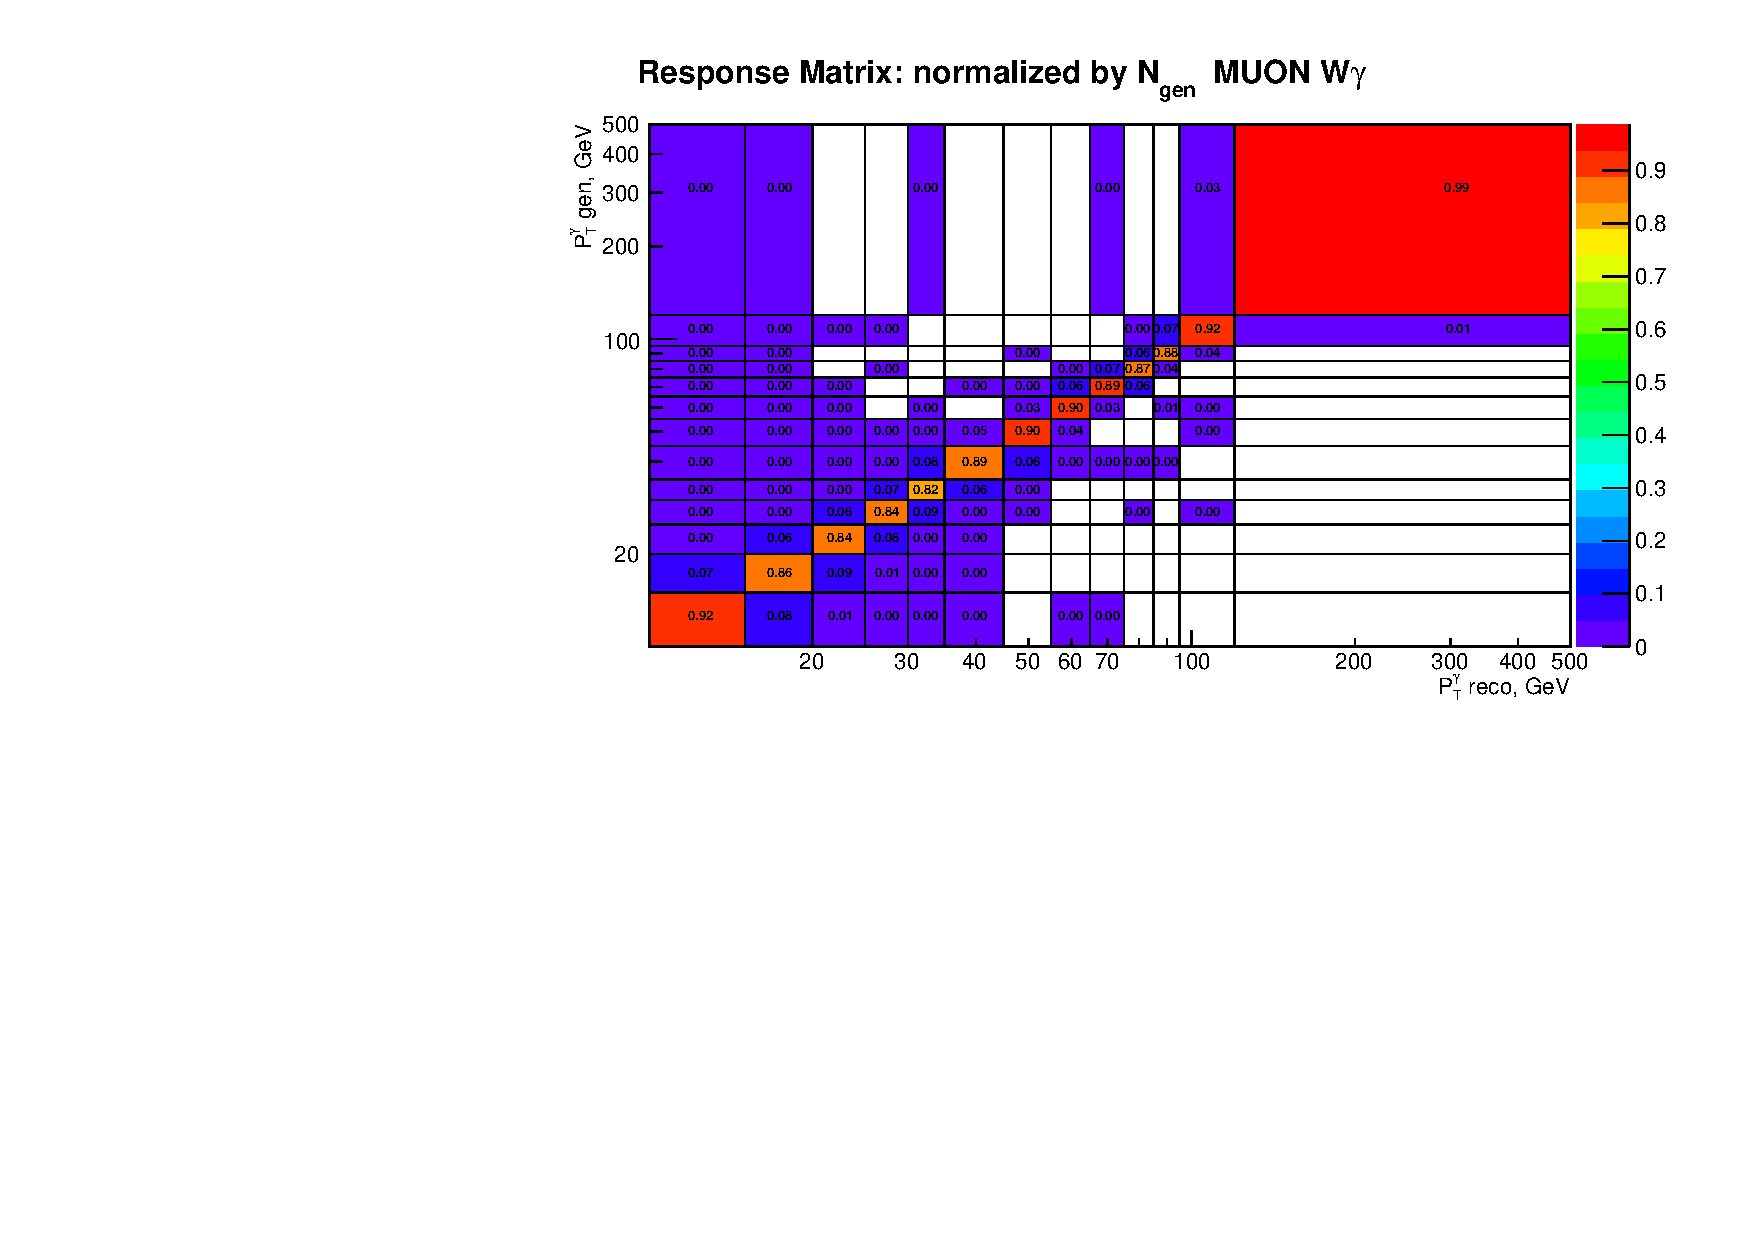
\includegraphics[width=0.89\textwidth]{../figs/figs_v11/MUON_WGamma/Constants/cResponseMatr_MUON_WGamma__yield_pm_stat.pdf}\\
  \label{fig:respMatrices_Wg}
  \end{center}
\end{figure}
\end{frame}%{Detector Resolution Unfolding}

\begin{frame}\frametitle{Correlation Matrices for Unfolded Yields. Muon channel}
\scriptsize Correlation matrix on the unfolded yields (not on cross section), takes into account statistical error only (correlation matrices for the systematic errors are prepared separately).
\begin{figure}[htb]
  \begin{center}
   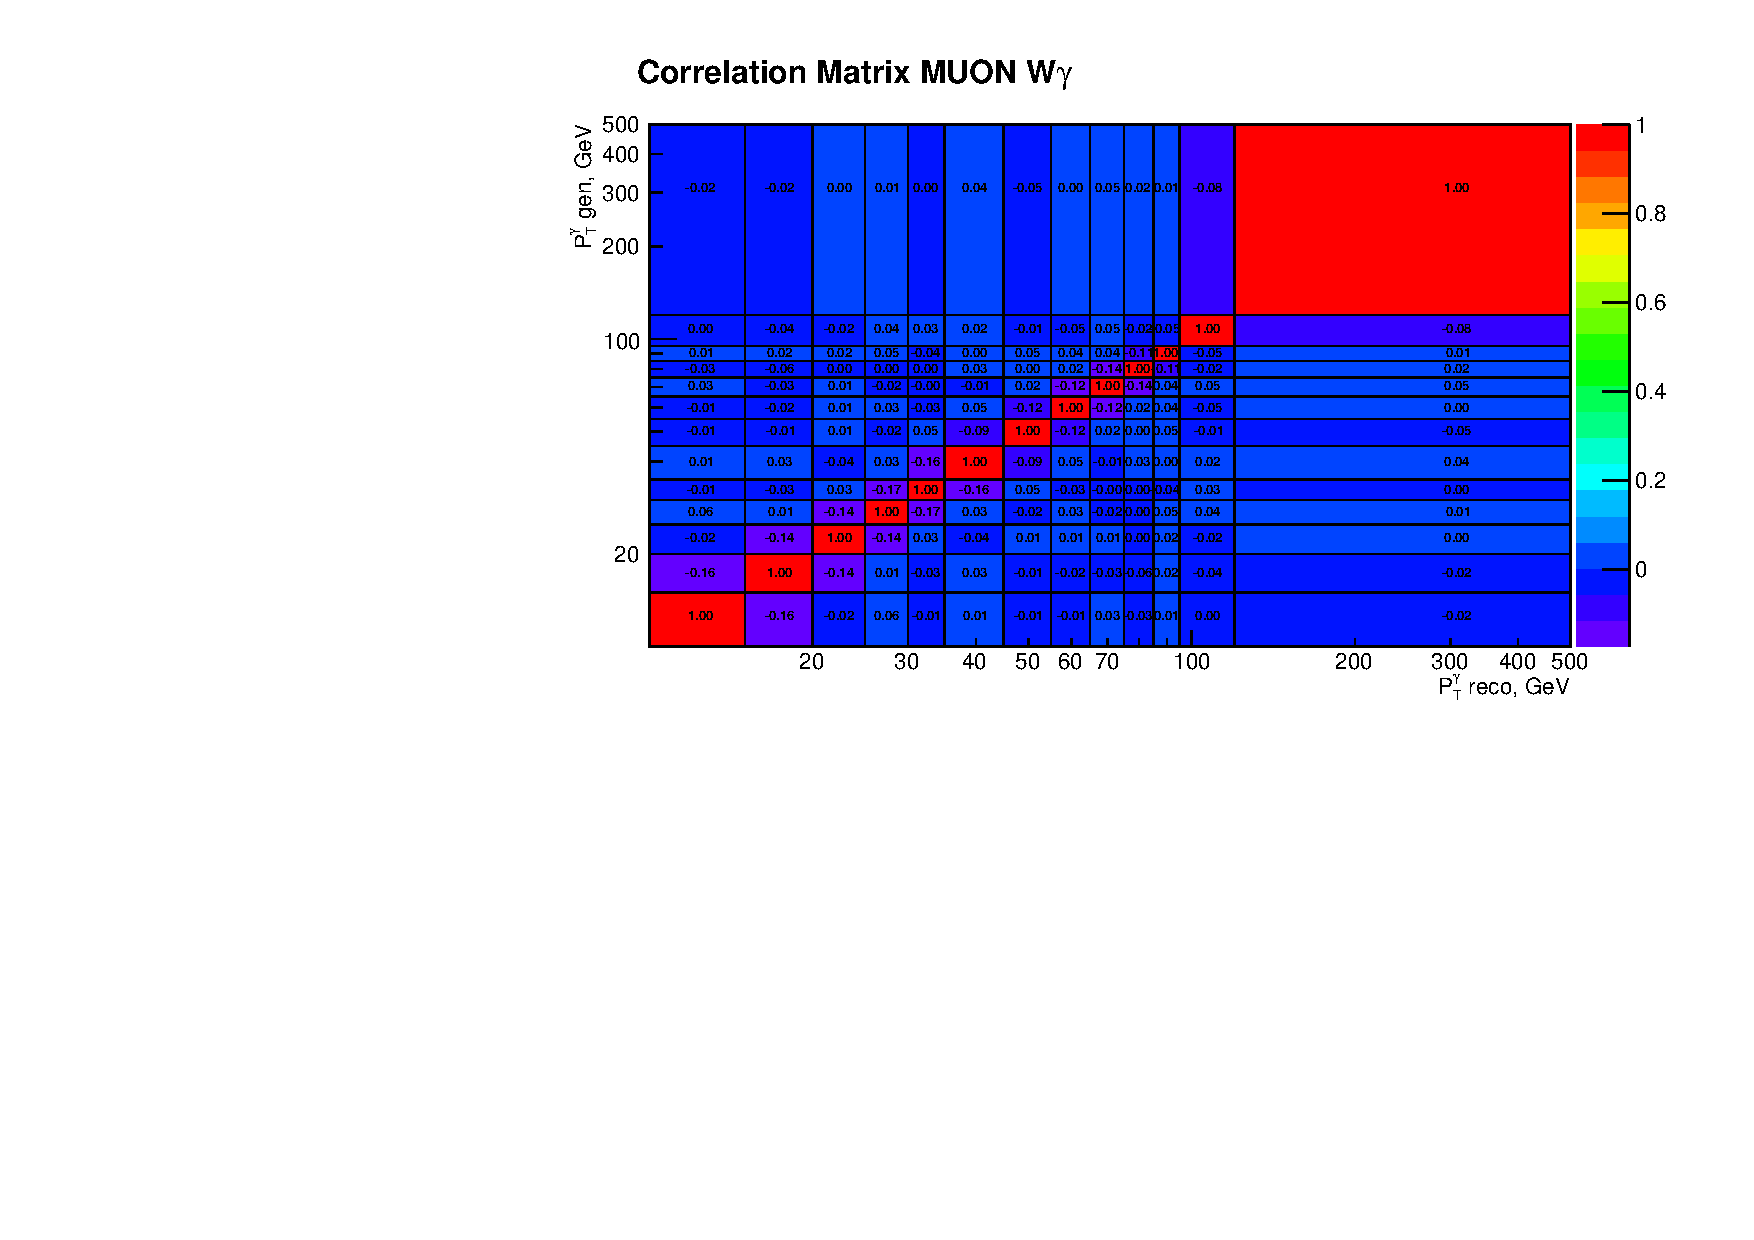
\includegraphics[width=0.89\textwidth]{../figs/figs_v11/MUON_WGamma/Constants/matrCorrelation_yield_pm_stat.pdf}\\
  \label{fig:covMatrices_Wg}
  \end{center}
\end{figure}
\end{frame}%{Correlation Matrices on Unfolded Yields}

\begin{frame}\frametitle{Acc x Eff Correction. Method Description}
\begin{itemize}
  \item {\footnotesize{Computed as combined value bin-by-bin based on signal MC}}
  \item {\footnotesize\bfseries{Numerator:}}
  \begin{itemize}
     \scriptsize
     \item For total cross section: selected signal MC yields with PU weight applied
     \item For differential cross section: selected signal MC yields with PU weight applied in $p_T^{\gamma}$ GEN bins 15-20-25... Transition to $p_T^{\gamma}$ RECO bins performed with unfolding
  \end{itemize}
  \item {\footnotesize\bfseries{Denominator:}}
  \begin{itemize}
     \scriptsize
     \item For each event in unskimmed signal MC file, photon and lepton (two leptons for Z$\gamma$) which refer to W$\gamma$ (Z$\gamma$) and determine $\Delta{R}$ GEN and $p_T^{\gamma}$ GEN
     \item For total cross section: calculate number of events within phase space cut
     \item For differential cross section: calculate number of events within phase space cut in 15-20-25... $p_T^{\gamma}$ GEN bins
  \end{itemize}
\end{itemize}
\end{frame}%{Acc x Eff. Method Description}
